\documentclass[letterpaper]{article} % DO NOT CHANGE THIS
\usepackage[submission]{aaai2027}  % DO NOT CHANGE THIS (anonymous, double-blind)
% The serif, sans-serif, and monospaced fonts are loaded automatically by
% aaai2027.sty (newtxtext, helvet, courier). DO NOT add any font package.
\usepackage[hyphens]{url}  % DO NOT CHANGE THIS
\usepackage{graphicx} % DO NOT CHANGE THIS
\urlstyle{rm} % DO NOT CHANGE THIS
\def\UrlFont{\rm}  % DO NOT CHANGE THIS
\usepackage{natbib}  % DO NOT CHANGE THIS AND DO NOT ADD ANY OPTIONS TO IT
\usepackage{caption} % DO NOT CHANGE THIS AND DO NOT ADD ANY OPTIONS TO IT
\frenchspacing  % DO NOT CHANGE THIS
\usepackage{booktabs}
\usepackage{amsmath}
\usepackage{amssymb}
\pdfinfo{
/TemplateVersion (2027.1)
}
% Double-blind: no build date, time zone or TeX banner in the PDF metadata.
\pdfinfoomitdate=1
\pdftrailerid{}
\pdfsuppressptexinfo=-1

\setcounter{secnumdepth}{2}
\hyphenation{DENSEWORLD}

% AAAI-27 Bridge "Modeling and Simulating Human Behavior in the Age of AI: From Cognition to
% Society" (Cog2Soc). Rules (cog2soc.github.io, read 2026-11-26): research findings, experience
% reports, methods, theory, datasets, evaluation tools, demos, position papers; at most 4 pages
% EXCLUDING references, AAAI two-column format; anonymized for double-blind review; at least two
% reviews on relevance, substance, suitability for discussion; non-archival; OpenReview
% AAAI.org/2027/Bridge/Cog2Soc. The call asks each paper to explain the human phenomenon, the
% approach or research question, and the connection to another participating community.
% Deadline Nov 29 2026 23:59 AoE (= Nov 30 03:59 PST); notification Dec 10 2026 AoE.
% Dual submission is not stated: this work is also an AAAI-27 student abstract (non-archival)
% and is under review at Human-Centric AgMS; disclose both on OpenReview.
% v3 (2026-11-27) = v2 plus the fixes of the fresh Claude judge, round 1 (51/100), see
% ../v2_Cog2Soc/TODOs.md. Facts follow the code, not earlier drafts:
%  * the method is the 3-stage factor-clip curriculum of src/m09c1_surgery_encoder.py with
%    configs/train/surgery_3stage_DI_diheavy_encoder.yaml (layout, agent, interaction clips;
%    blocks [0,4) then [0,8) of 48 unfrozen; predictor trained; frozen teacher; SPD; 50% raw
%    replay; epoch split 0.30/0.25/0.45). There is NO factorized predictor, dictionary, visibility
%    gate or covariance penalty in the code, so none is described.
%  * RAW = the same recipe on raw clips (configs/train/surgery_raw_encoder.yaml).
%  * Table 2 numbers: results/*.json (copied from outputs/workshop/attribution_10k, src/utils/paired_ladder.py).
%  * no face or plate blurring exists in src/ or scripts/, so no such claim is made.
%  * factor clips come from Grounding DINO + SAM 3 (src/m10_sam_segment.py, src/m11_factor_datasets.py);
%    Causal L1 predicts the 2nd temporal half from the 1st (src/utils/pt_causal.py); the split is
%    clip-level (src/utils/clip_splits.py); Ours is ONE fixed arm in every cell of Table 1.

\title{FactorJEPA on DENSEWORLD-115k: Can a World Model Predict Crowded, Chaotic South Asian Streets?}

\author{Anonymous Submission}
\affiliations{}

\begin{document}

\maketitle

\begin{abstract}
On a crowded South Asian street, pedestrians, two-wheelers, auto-rickshaws, carts, and animals share one right of way and coordinate by negotiation rather than lane rules, often while partly hidden from each other. Models of such collective behaviour are often calibrated on sparser, lane-structured, mostly Western scenes. We contribute DENSEWORLD-115k, 115,687 clips (276 hours) from 714 public YouTube videos of 22 Indian cities, released as reconstructible metadata, and FactorJEPA, a curriculum that adapts the video world model V-JEPA 2.1 first on clips of the street layout, then on the road users, then on their interactions. Compared with seven adaptation methods under identical clips and budgets, one fixed FactorJEPA configuration predicts masked and future content better at both 2B and 1B scale, and after full 115k-clip training it separates from the stronger of the two rivals trained at that scale on all four diagnostics of predictive structure, by 13.9 to 43.3 widths of the paired 95\% confidence interval. An ablation on raw clips shows that the staged adaptation carries most of this gain, while the layout, agent, and interaction clips make prediction more robust when more of the scene is hidden. Competing methods still lead on temporal coherence. We discuss what this offers the modelling and cross-cultural evaluation of collective behaviour.
\end{abstract}

\begin{links}
    \link{Dataset}{https://huggingface.co/datasets/anonymousML123/denseworld-115k}
\end{links}

\section{Introduction}

\paragraph{The human phenomenon.} On South Asian streets, road edges are negotiated rather than painted, pedestrians and vehicles of very different speeds share one right of way, clutter keeps road users partly hidden, and who goes first is settled by local norms more than by lane rules. The coordination shows in observable behaviour: one road user yields to another by slowing or swerving, pedestrians accept gaps in moving traffic, and vehicles pass each other at small lateral distances. Behaviour models from transport research and computational social science, such as social-force and agent-based models \cite{helbing1995social}, describe these behaviours with hand-set interaction rules calibrated on observed data, which often comes from sparser, lane-structured scenes. Large driving datasets such as BDD100K \cite{yu2020bdd100k} and nuScenes \cite{caesar2020nuscenes} sample this regime rarely.

\paragraph{Our approach.} We ask whether a video world model can learn this collective behaviour directly from street video. Joint Embedding Predictive Architectures (JEPA) such as V-JEPA 2.1 \cite{murlabadia2026vjepa21} learn without labels by predicting masked or future video content as embeddings rather than pixels. Agent-based models are typically built in layers: the environment, then the individuals, then their interactions. We adapt V-JEPA 2.1 in the same order. We contribute:
\begin{itemize}
    \item \textbf{DENSEWORLD-115k}, a 276-hour drive-through, walk-through, and aerial video corpus of 22 Indian cities, released as reconstructible metadata.
    \item \textbf{FactorJEPA}, a three-stage curriculum that adapts V-JEPA 2.1 on layout, agent, and interaction clips derived automatically from the video, with no extra inputs at inference.
    \item A controlled comparison with seven adaptation methods at two model and two data scales on all 13 diagnostics, wins and losses alike, and an ablation that separates the staged adaptation from the curriculum's clips.
\end{itemize}

\begin{figure*}[t]
\centering
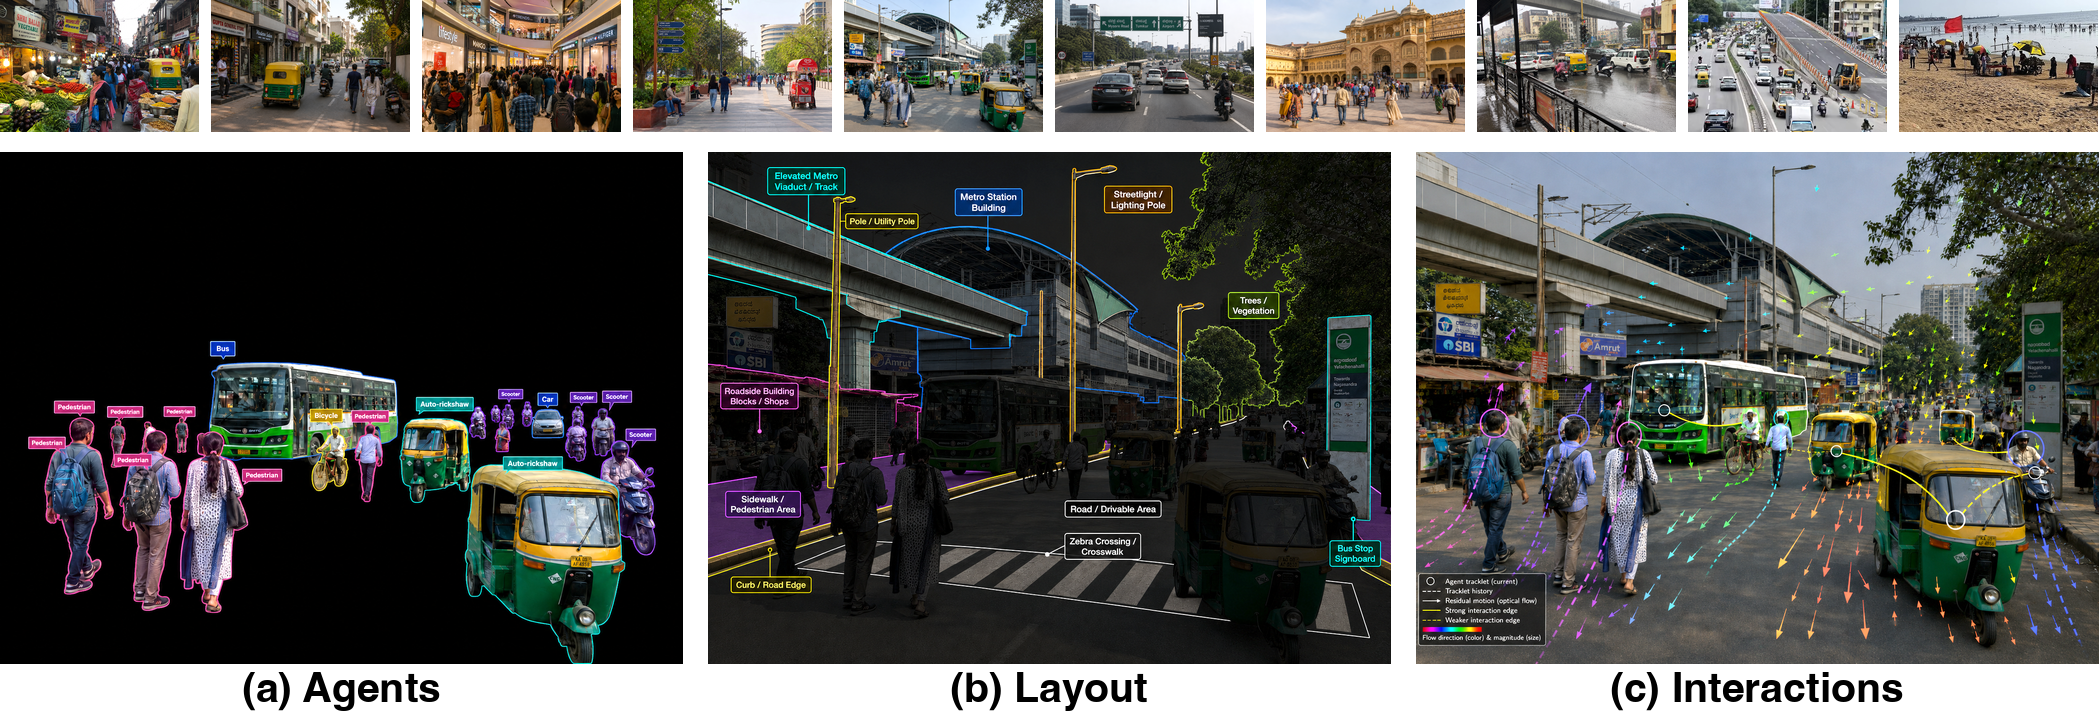
\includegraphics[width=\textwidth]{figures/denseworld_teaser.png}
\caption{DENSEWORLD-115k. Top: ten scene types, left to right: market, residential, commercial, promenade, transit, highway, heritage, junction, flyover, and beach. Bottom: an illustration of the three clip types FactorJEPA trains on: (a) road users with the background suppressed, (b) the layout with road users suppressed, and (c) interactions between tracked road users (circles: road users; arrows: motion, colour for direction and length for magnitude; solid or dashed edges: stronger or weaker coupling).}
\label{fig:teaser}
\end{figure*}

\section{DENSEWORLD-115k}

DENSEWORLD-115k records everyday street behaviour in 22 Tier-1 and Tier-2 Indian cities: 115,687 clips of 4 to 10 seconds (276 hours; Figure~\ref{fig:teaser}, top), cut with scene and shot-boundary detection from 714 public long-form YouTube videos (480p). It covers drive-through, walk-through, and aerial viewpoints across markets, residential lanes, transit corridors, junctions, flyovers, heritage sites, and beaches, at different times of day and in different weather. For 86,831 clips an automatic pipeline finds the road users: Grounding DINO \cite{liu2024groundingdino} detects them on anchor frames, SAM~3 \cite{carion2025sam3} tracks their masks through the clip, and pairs of road users that are close and move relative to each other are marked as interactions.

\begin{figure}[t]
\centering
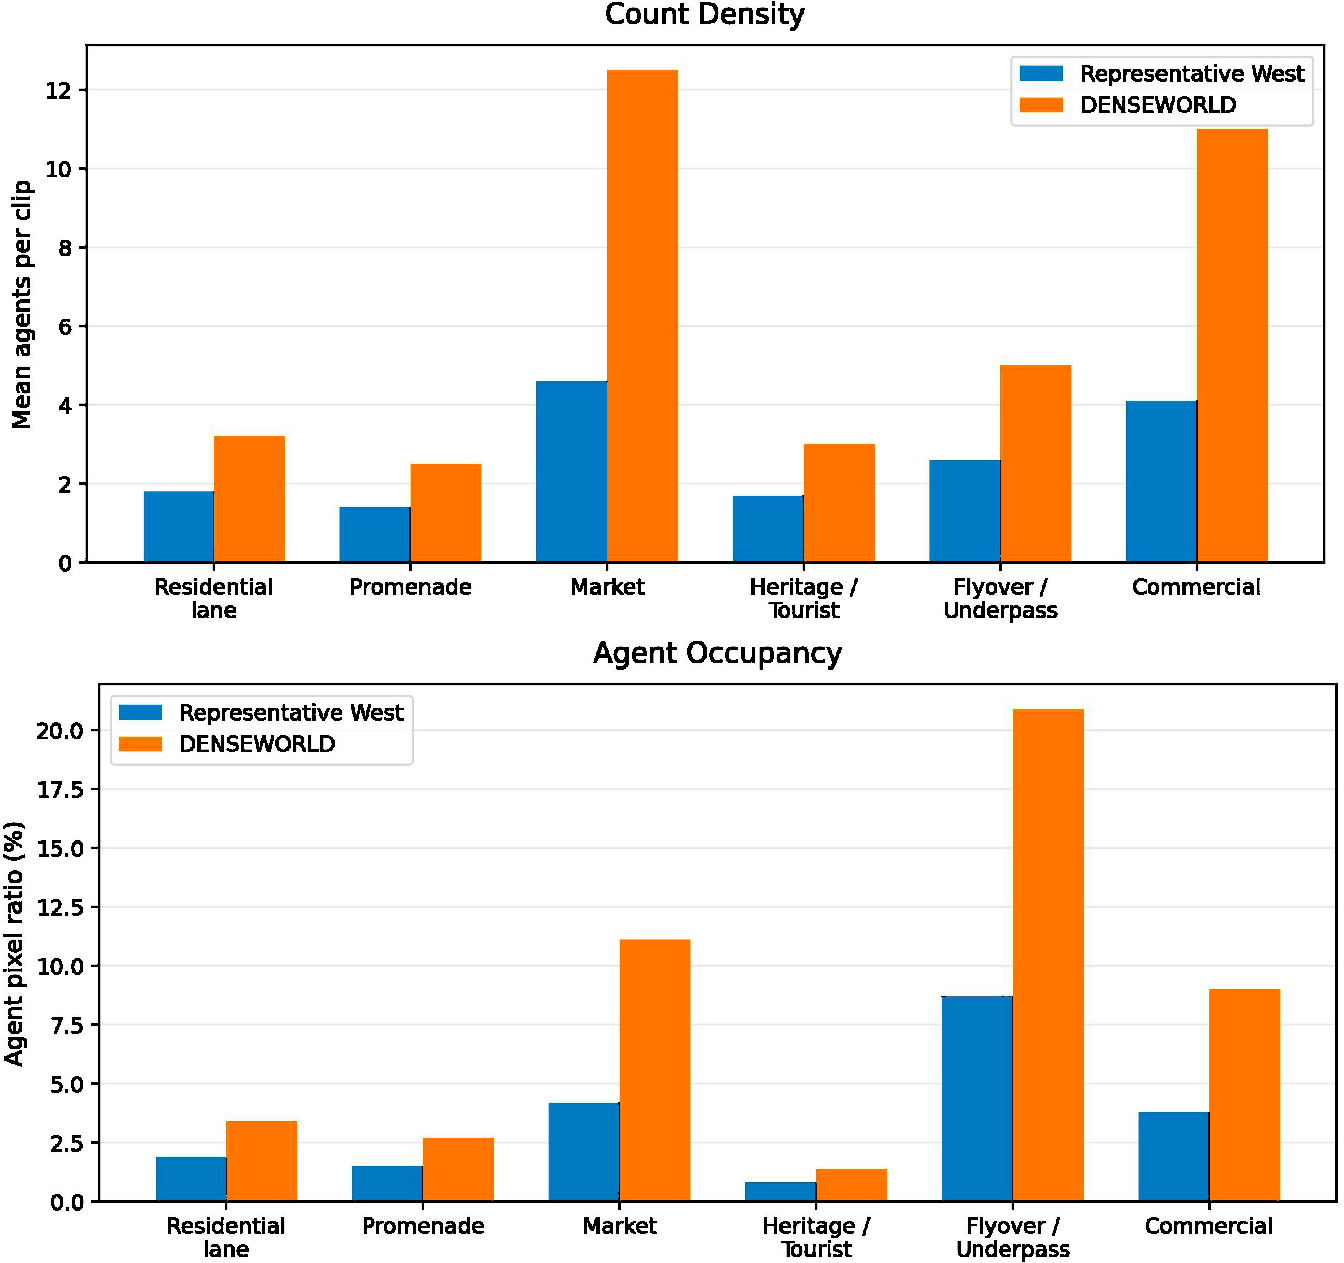
\includegraphics[width=\columnwidth]{figures/denseworld_vs_west_density_bold.pdf}
\caption{Mean agents per clip (top) and share of pixels covered by agents (bottom) for DENSEWORLD and a Western reference drawn from BDD100K and nuScenes, per scene type.}
\label{fig:density}
\end{figure}

Against a reference set of BDD100K and nuScenes clips grouped by the same scene types, DENSEWORLD has more agents per clip and a larger share of pixels covered by agents on each of the six types compared (Figure~\ref{fig:density}). These two axes are the ones measured here; occlusion and interaction pressure are the natural next axes. The gap lies in the data itself: a behaviour model calibrated on the Western reference would meet denser scenes here on all six types.

\paragraph{Release and responsible use.} Respecting the creators' copyright, the release ships the source list, the clip manifest with timestamps, and a deterministic script that rebuilds every clip from YouTube, rather than the videos, under a CC BY 4.0 licence for the metadata. Rebuilt clips are the public videos as posted, so a video its creator removes can no longer be rebuilt, and rights holders can ask on the dataset page for a source to be removed. The people filmed did not consent individually, so the data is meant for research on aggregate street behaviour, not on individuals.

\section{FactorJEPA}

FactorJEPA keeps V-JEPA 2.1's encoder, predictor, masking policy, and prediction objective, and changes what the model is trained on and which blocks it updates. From a checkpoint already adapted to the corpus by plain continued pretraining, it trains in three stages on clips built from the automatic masks (Figure~\ref{fig:teaser}, bottom): layout clips in which every detected road user is blurred; then agent clips in which the background is suppressed, mixed 70/30 with layout clips; then interaction clips, cropped around pairs of interacting road users, mixed 70/15/15 with the other two. Half of the training samples are raw clips, which keeps the model anchored to ordinary video. The first stage unfreezes the first 4 of the encoder's 48 blocks and the later stages the first 8, following surgical fine-tuning \cite{lee2023surgical}; the predictor trains throughout against a frozen teacher, selective projection decay \cite{tian2024spd} keeps the weights near their starting point, and the fixed configuration splits its epochs 30/25/45 across the stages. At inference FactorJEPA is an ordinary V-JEPA model: no detector, tracker, or mask is needed. Unlike SlotFormer's object-centric slots \cite{wu2023slotformer} and DriveWorld's split of static scene from dynamics \cite{min2024driveworld}, FactorJEPA keeps one predictor and builds the layout, agent, and interaction structure into what it trains on.

\section{Evaluation}

\paragraph{Protocol.}
We adapt V-JEPA 2.1 at 2B and 1B parameters on a stratified 10k-clip set, and the 1B model also on the full corpus. FactorJEPA is compared with the frozen backbone, full fine-tuning, linear probing then fine-tuning, continual self-supervised learning, LoRA \cite{hu2022lora}, DoRA \cite{liu2024dora}, and Auto-RGN \cite{lee2023surgical}, all under identical clips, masking, optimization steps, and splits. Test clips are held out at the clip level (1,825 in the 10k regime, 23,106 in the full regime), so a source video can contribute clips to both training and test (Section~\ref{sec:scope}). Every margin is a paired 95\% BCa bootstrap interval over test clips.

\paragraph{Diagnostics of predictive structure.}
\emph{Future-frame L1}: error between predicted and target-encoder embeddings on the token blocks hidden by V-JEPA's mask generator. \emph{Causal L1}: the same error when the second half of a clip is predicted from its first half. \emph{Mask-ratio slope}: growth of that error as the hidden fraction rises from 0.3 to 0.9. \emph{Motion cosine}: how well a linear probe recovers clip motion from the embedding. Nine further diagnostics probe temporal coherence and semantics (Table~\ref{tab:headline}).

\begin{table}[t]
\centering
\small
\setlength{\tabcolsep}{2pt}
\begin{tabular}{lrrrrrr}
\toprule
 & \multicolumn{2}{c}{2B$\cdot$10k} & \multicolumn{2}{c}{1B$\cdot$10k} & \multicolumn{2}{c}{1B$\cdot$115k} \\
\cmidrule(lr){2-3}\cmidrule(lr){4-5}\cmidrule(lr){6-7}
Diagnostic & Ours & Rival & Ours & Rival & Ours & Rival \\
\midrule
future-frame L1 ($\downarrow$) & \textbf{0.496} & 0.504\textsuperscript{L} & \textbf{0.590} & 0.596\textsuperscript{L} & \textbf{0.573} & 0.589\textsuperscript{L} \\
causal-block L1 ($\downarrow$) & \textbf{0.529} & 0.533\textsuperscript{L} & \textbf{0.614} & 0.617\textsuperscript{L} & \textbf{0.597} & 0.607\textsuperscript{L} \\
mask-ratio slope ($\downarrow$) & \textbf{0.053} & 0.054\textsuperscript{L} & \textbf{0.052} & 0.053\textsuperscript{D} & \textbf{0.047} & 0.058\textsuperscript{L} \\
motion-cos ($\uparrow$) & 0.116 & \textbf{0.244}\textsuperscript{F} & 0.048 & \textbf{0.090}\textsuperscript{F} & \textbf{0.097} & 0.078\textsuperscript{L} \\
\midrule
temporal-order ($\uparrow$) & 0.944 & \textbf{0.947}\textsuperscript{Z} & 0.925 & \textbf{0.927}\textsuperscript{C} & \textbf{0.918} & 0.915\textsuperscript{Z} \\
pace ($\uparrow$) & 0.719 & \textbf{0.724}\textsuperscript{L} & 0.711 & \textbf{0.729}\textsuperscript{Z} & 0.703 & 0.703\textsuperscript{L} \\
action top-1 ($\uparrow$) & 0.500 & \textbf{0.528}\textsuperscript{C} & 0.483 & \textbf{0.509}\textsuperscript{F} & 0.567 & \textbf{0.572}\textsuperscript{L} \\
arrow-of-time ($\uparrow$) & 0.935 & \textbf{0.965}\textsuperscript{Z} & 0.957 & \textbf{0.965}\textsuperscript{Z} & 0.955 & \textbf{0.975}\textsuperscript{Z} \\
TCC $\tau$ ($\uparrow$) & 0.274 & \textbf{0.292}\textsuperscript{Z} & 0.287 & \textbf{0.334}\textsuperscript{Z} & 0.380 & \textbf{0.400}\textsuperscript{Z} \\
exposure-bias ($\downarrow$) & 0.048 & \textbf{0.038}\textsuperscript{C} & \textbf{0.034} & 0.036\textsuperscript{D} & 0.038 & \textbf{0.035}\textsuperscript{L} \\
rollout drift ($\downarrow$) & 0.011 & \textbf{0.008}\textsuperscript{C} & 0.005 & 0.005\textsuperscript{D} & 0.007 & \textbf{0.006}\textsuperscript{L} \\
L1-vs-$\Delta t$ ($\downarrow$) & 0.008 & \textbf{0.006}\textsuperscript{C} & 0.009 & \textbf{0.007}\textsuperscript{Z} & 0.009 & \textbf{0.007}\textsuperscript{Z} \\
TCC cycle ($\downarrow$) & 2.249 & \textbf{2.111}\textsuperscript{Z} & 2.416 & \textbf{2.195}\textsuperscript{Z} & 2.806 & \textbf{2.132}\textsuperscript{Z} \\
\bottomrule
\end{tabular}
\par\smallskip
{\small\raggedright
Rival superscript: L LoRA, D DoRA, F full fine-tuning, C continual self-supervised learning, Z frozen backbone. At 115k only LoRA and the frozen backbone were trained as rivals.\par}
\caption{One fixed FactorJEPA model (Ours, identical in every cell) against its strongest rival on 13 diagnostics. Above the rule: the four diagnostics of predictive structure; below: nine diagnostics of temporal coherence and semantics, where the rival leads on most rows. Bold: the better of each pair (neither when equal).}
\label{tab:headline}
\end{table}

\begin{figure}[!tb]
\centering
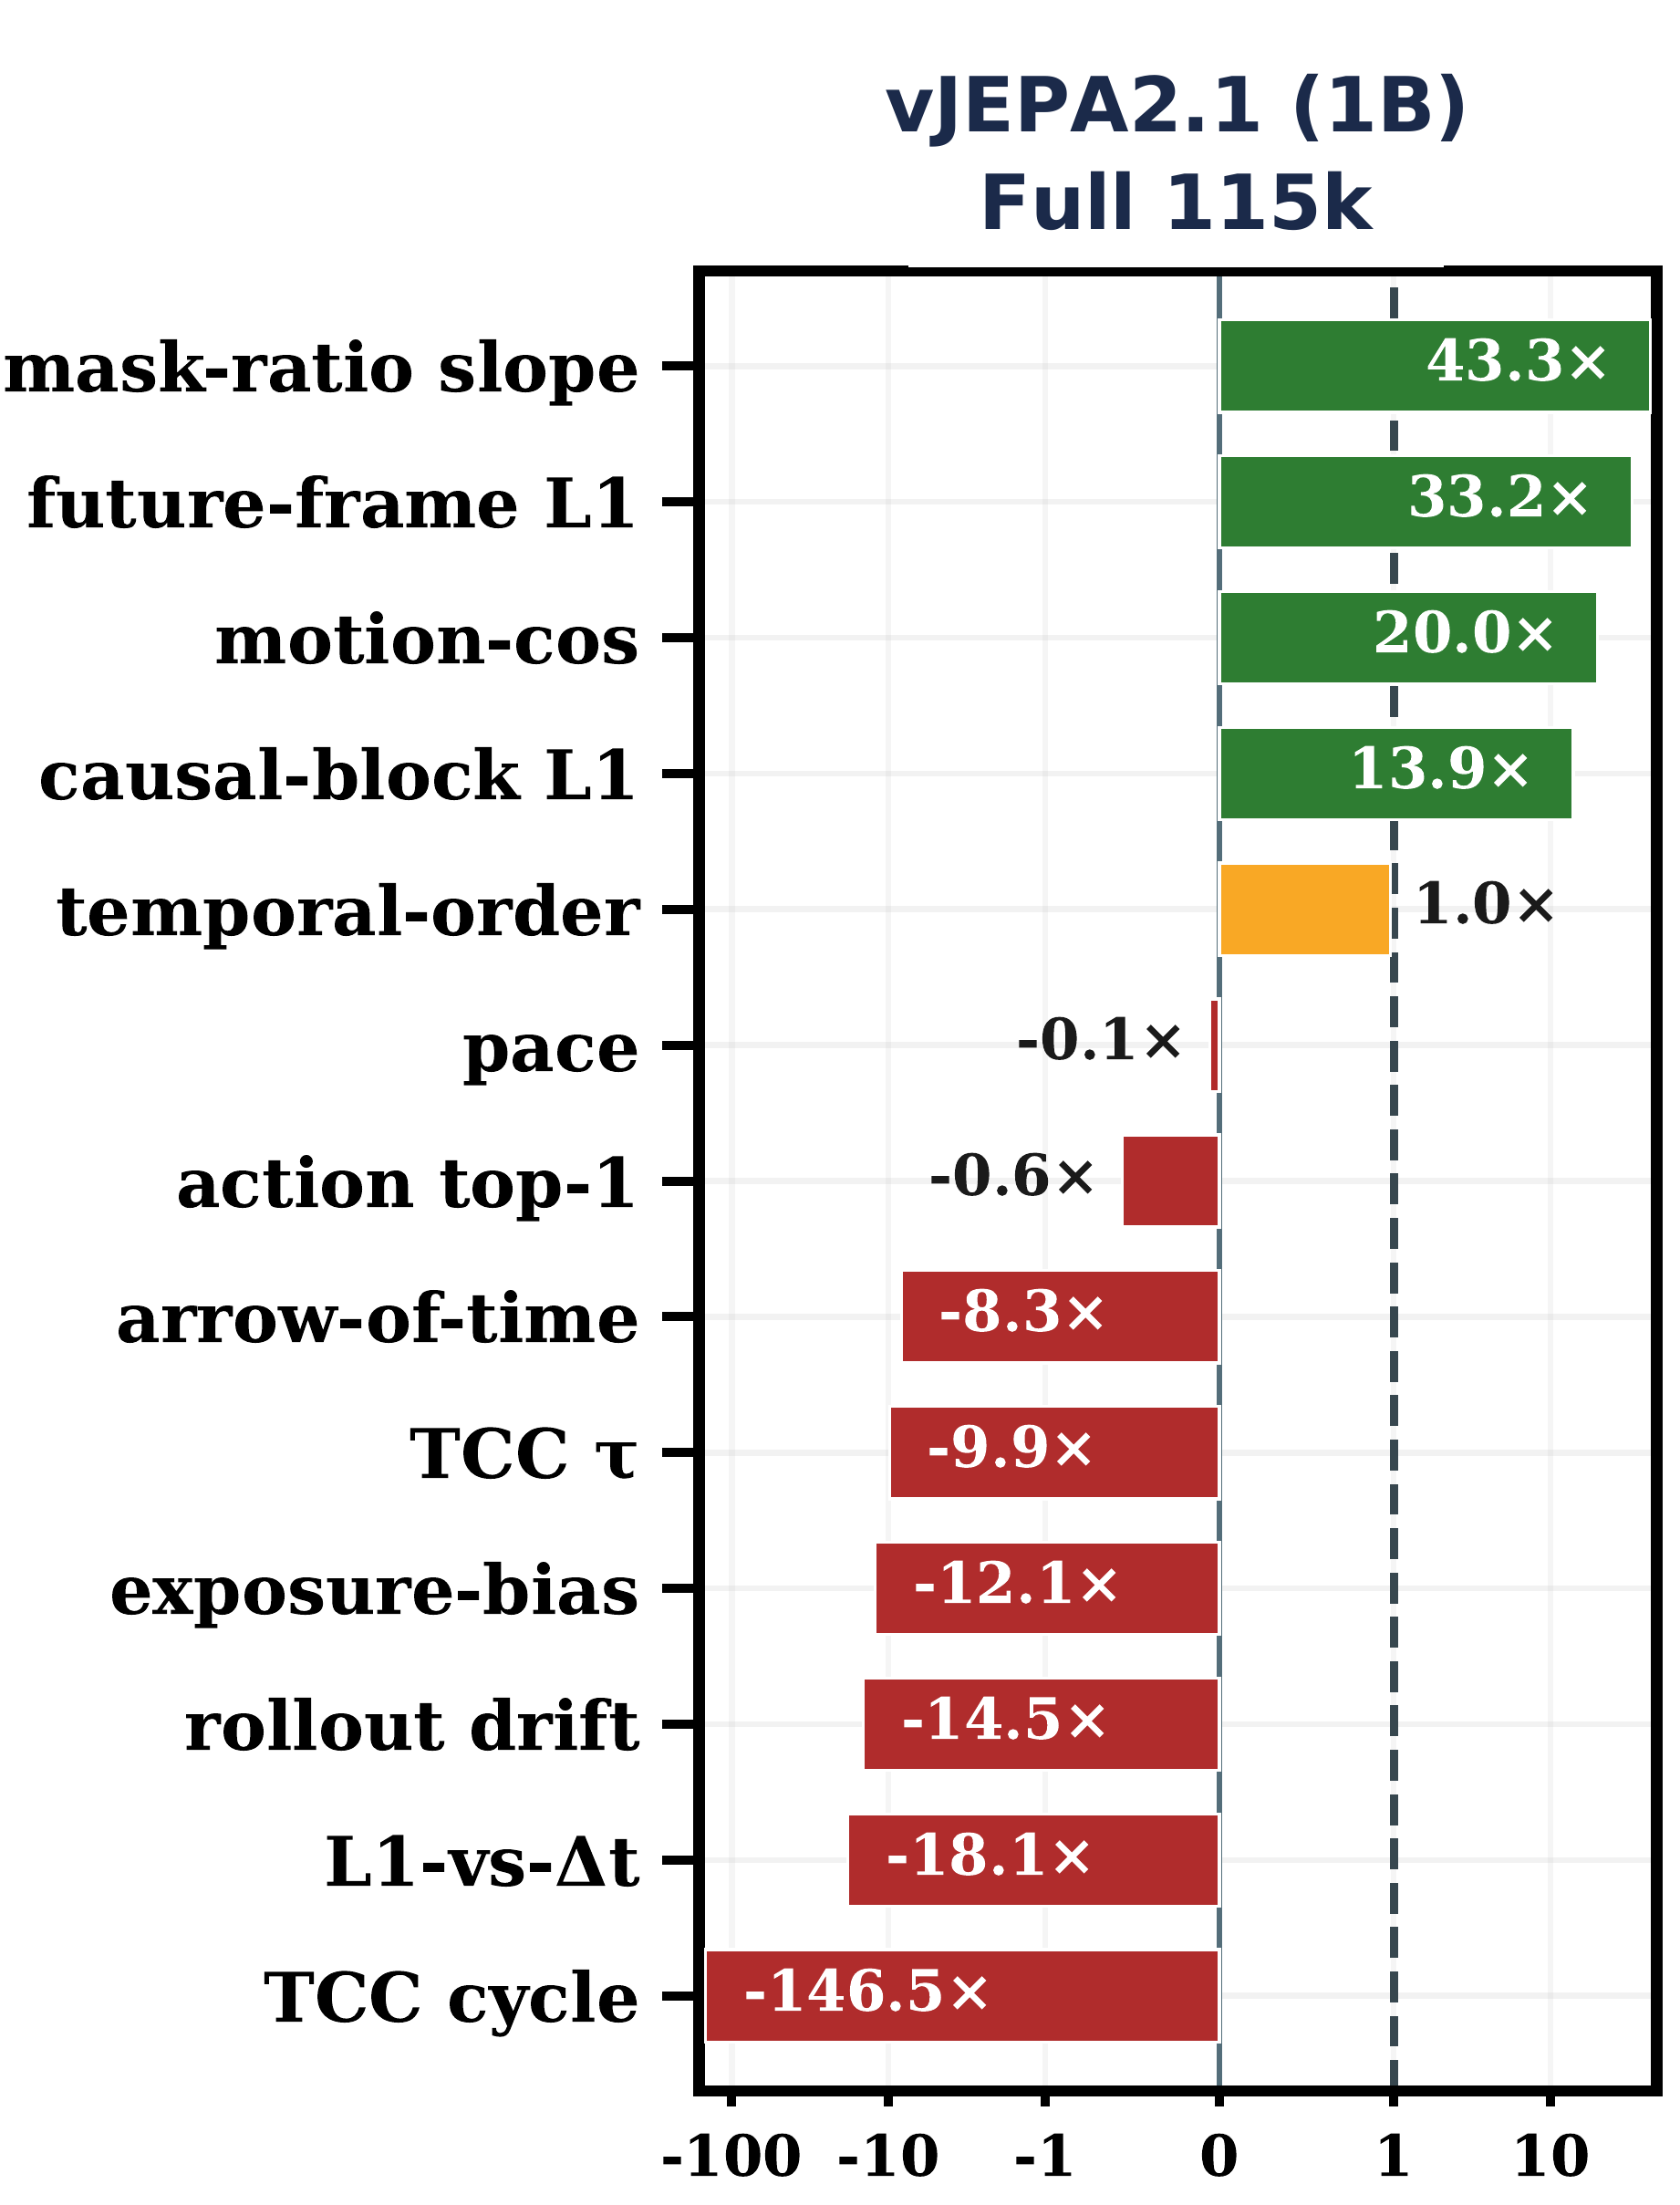
\includegraphics[width=0.97\columnwidth]{figures/forest_115k_col.png}
\caption{Separation of the fixed FactorJEPA model from the strongest rival at 1B on the full corpus, in widths of the paired 95\% BCa interval (symmetric-log axis). Green: FactorJEPA ahead by at least one width; yellow: ahead within the interval; red: the rival ahead.}
\label{fig:forest}
\end{figure}

\paragraph{Findings.}
With limited data (Table~\ref{tab:headline}), FactorJEPA separates from the best rival on Future-frame L1 and Causal L1 at both scales and on Mask-ratio slope at 1B, while Motion cosine favors full fine-tuning. After full 115k-clip training, against the two rivals trained at that scale (LoRA and the frozen backbone), FactorJEPA separates on all four diagnostics, Motion cosine included (Figure~\ref{fig:forest}), by 13.9 (Causal L1) to 43.3 (Mask-ratio slope) interval widths, a 2.7\% lower Future-frame L1 and a 19\% flatter Mask-ratio slope than LoRA. Full fine-tuning, which leads on Motion cosine at 10k, was not trained at 115k, so whether more data closes that gap remains open. Method rankings on the four diagnostics replicate from the 2B to the 1B backbone (Spearman $\rho \geq 0.895$). On the diagnostics below the rule, the best rival leads at 115k on six (rollout drift, exposure bias, L1-versus-$\Delta t$ decay, arrow-of-time, and the two TCC measures) by 8.3 to 146.5 interval widths. FactorJEPA's gain is in one-step prediction of crowded scenes; on the coherence of long predicted futures, the rivals still lead.

\begin{table}[t]
\centering
\small
\setlength{\tabcolsep}{3pt}
\begin{tabular}{llrrrr}
\toprule
 & Adaptation & Fut.\ L1$\downarrow$ & Causal$\downarrow$ & Mask$\downarrow$ & Motion$\uparrow$ \\
\midrule
2B & plain & 0.533 & 0.558 & 0.0625 & \textbf{0.151} \\
 & RAW & 0.497 & \textbf{0.528} & 0.0565 & 0.133 \\
 & Ours & \textbf{0.496} & 0.529 & \textbf{0.0531} & 0.116 \\
\midrule
1B & plain & 0.607 & 0.628 & 0.0586 & 0.054 \\
 & RAW & \textbf{0.587} & \textbf{0.611} & 0.0528 & \textbf{0.060} \\
 & Ours & 0.590 & 0.614 & \textbf{0.0515} & 0.048 \\
\bottomrule
\end{tabular}
\caption{Where the gain comes from, 10k clips, 1,825 test clips. Plain: continued pretraining, the starting point of both other rows. RAW: the same staged adaptation as Ours on raw clips only. Ours: the staged adaptation on the curriculum's layout, agent, and interaction clips. Every RAW-minus-plain and Ours-minus-RAW difference excludes zero at 95\% under both clip and source-video resampling (127 videos), except Future-frame L1 at 2B.}
\label{tab:ladder}
\end{table}

\paragraph{Where the gain comes from.} Table~\ref{tab:ladder} separates the two parts of FactorJEPA. The staged adaptation carries most of the gain: on raw clips alone it lowers Future-frame L1 by 0.036 (2B) and 0.020 (1B) below plain continued pretraining, and it already beats LoRA on Future-frame and Causal L1 at both scales. The layout, agent, and interaction clips then flatten the Mask-ratio slope at both scales (by 6\% at 2B and 2\% at 1B), so prediction degrades more slowly as more of the scene is hidden, which is the situation of occluded road users. They cost Motion cosine at both scales and a little prediction error: 0.001 in Causal L1 at 2B and about 0.003 in Future-frame and Causal L1 at 1B. Most of the gain therefore does not depend on the automatic labels, and what the labels buy is a specific property: robustness to missing evidence.

\section{What This Offers Models of Collective Behaviour}

Agent-based and social-force models write interaction rules by hand and fit their parameters to observed trajectories. FactorJEPA learns from raw street video in the order those models are built (environment, individuals, interactions), and our results already support the first part of that use: one-step prediction of crowded scenes improves at every scale and data size tested, and the clips that isolate layout, road users, and their interactions make the model degrade more slowly as road users are hidden. Temporal coherence over longer rollouts, which a simulation needs, is where the rivals still lead. Because the model needs only monocular public video, with no maps or sensors, it can be trained wherever street footage exists, which is what cross-cultural evaluation of behaviour models needs. For behaviour modellers, DENSEWORLD-115k offers a dense, non-Western reference corpus, and the curriculum offers a way to ask which kind of structure (layout, individuals, or interactions) a learned predictor needs.

\section{Scope and Next Steps}
\label{sec:scope}

Every diagnostic is measured in the frozen V-JEPA embedding space or with a linear probe on it. Trajectory forecasting, a comparison with a calibrated social-force or agent-based model, and a check of the interaction clips against human judgements of who yields to whom are the next tests; none is reported here, and the interaction clips are chosen by a proximity and relative-motion rule. The clip-level split lets a source video contribute to both training and test, and no city is held out. Video-level and city-level splits, dense-traffic regions beyond India (all footage here is Indian), and repeated training runs (each configuration was trained once) are the natural extensions.

{\small
\bibliography{factorjepa}
}

\end{document}
